% !TEX encoding = UTF-8
% !TEX TS-program = pdflatex
% !TEX root = ../Tesi.tex

%************************************************

%************************************************

Speech or text interaction between human beings and computers is gaining more and more popularity nowadays. People want to communicate with computers in the same manner as they communicate with other human beings. One of the main tools used for analyzing speech and providing human-like answers is Natural Language Processing (NLP). In order to provide suitable responses based on phrases or keywords taken from questions as well as to keep the communication continuous, there is a need to create a dialogue system or program, which is often called a chatbot or a chatterbot. The chatbot is a computer program that has the ability to communicate with people by providing answers to questions and holding the conversation using Natural Language Processing. People input the natural language speech or text, while the program should provide the most suitable intelligent response in the form of text or speech. As long as the communication continues, this process is repeated.

% 
% * <siciliani.lu@gmail.com> 2018-04-06T15:09:35.037Z:
% 
% > is being repeated
% is repeated
% 
% ^.
% * <siciliani.lu@gmail.com> 2018-04-06T15:08:49.012Z:
% 
% > an ability
% the ability
% 
% ^.
% * <siciliani.lu@gmail.com> 2018-04-06T15:07:15.934Z:
% 
% > the human and the computer 
% human beings and computers
% 
% ^.


\section{User eXperience}

This chapter gives an overview of UX, distinguishes it from the concept of experience and presents the current research status, definitions and viewpoints of UX. Definition, in theory, is easy since the ISO 9241-210:2010 standard defines UX as follows: \textit{"A person's perceptions and responses that result from the use and/or anticipated use of a product, system or service."} \cite{ergonomics2011}. Apparently the definition and meaning are not that easy since UX is an umbrella term \cite{instone2005}. In some studies UX is regarded as a synonym of UI (User Interface), whereas in other studies it might be usability or anything vaguely related to users and technology. The following is a selection of UX views from various sources:

% * <siciliani.lu@gmail.com> 2018-04-06T15:17:30.914Z:
% 
% > are
% "is" (non si riferisce a "selection"?)
% 
% ^.
% * <siciliani.lu@gmail.com> 2018-04-06T15:11:44.975Z:
% 
% > some
% La renderei più formale. Direi qualcosa tipo "In some studies UX is regarded as a synonym of UI,  whereas...."
% oppure "UX  is sometimes seen as a synonym of UI, ..."
% 
% ^.
% * <siciliani.lu@gmail.com> 2018-04-06T15:11:24.270Z:
% 
% > equal with
% equal to
% 
% ^.
% * <siciliani.lu@gmail.com> 2018-04-06T15:10:10.129Z:
% 
% > from experiences
% Forse meglio: "distinguishes it from the concept of experience" ?
% 
% ^.

\begin{itemize}
\item UX is dependent on the subject, object, and interaction between these two \cite{luojus2010}.
\item No amount of professionalism in UX can substitute for our being personally involved \cite{alben1997}.
\item UX varies between situations and may change over time \cite{hassenzahl2003}.
\end{itemize}

All the above statements strongly emphasize the role of the user and his or her demographics and abilities as well as the current context of the user.

As Hassenzahl stated \textit{"There is no guarantee that users will actually perceive and appreciate the product the way designers wanted it to be perceived and appreciated"} \cite{hassenzahl2003}.

So what is the the difference between experience or user experience? 

Roto has taken a similar approach in her dissertation when she separates UX from experiences: \textit{“I claim that user experience is a special case of experience, where the person can use a system, with or without a purpose. Using means that the user not only senses the system, but also has the opportunity to manipulate or control the system. The system is a product, object, or a set of them; service systems often involve a human being such as a librarian. If there is no system at all, or if the person cannot control the system, we should use the term experience instead of user experience.”} \cite{roto2006}.



\section{Conversational User Interfaces}

In the Oxford English Dictionary a conversation is defined as a talk, especially an informal one, between two or more people, in which news and ideas are exchanged. This definition suggests that initiative belongs to both sides of the conversation, Radlinski and Craswell \cite{radlinski2017} calls this mixed initiative. Even though it is in the most recent years that conversational interfaces have gained widespread usage, they have been around for many years. Starting in the 60's with text-based dialogue systems for questions and answers, and chatbots that simulated natural conversations \cite{mctear2016}. Voice-based systems began to appear in the late 80's and spoken dialog technology became a key area of research within the speech and language communities \cite{mctear2016}. At the same time Voice User Interface (VUI) started to emerge and social robots that could mimic human expressions were developed. These human-like systems were developed in order to provide a more engaging interaction \cite{mctear2016}. According to Radlinski and Craswell \cite{radlinski2017} a conversational system is an information retrieval system that permits a mixed-initiative between an agent and user, where the agent's actions are based on the conversation, using both short and long term knowledge of the user. They further discuss that a conversational system needs to have at least five properties:


\begin{itemize}
\item \textit{User Revealment} - the system helps the user to express their needs.
\item \textit{System Revealment} - the system is clear with its capabilities to form user expectation of the system.
\item \textit{Mixed Initiative} - both system and user can take initiative for conversation.
\item Memory - the user can reference past statements and the system understands.
\item \textit{Set Retrieval} - The system can reason about the utility of sets of complementary items.
\end{itemize}


\subsection{Voice User Interfaces}

A VUI is what a user interacts with when communicating with a device or system using their voice \cite{cohen2004, mctear2016}. Even though it is in the most recent years that speech recognition technology has gained wide spread usage, it has been around for almost a century \cite{cohen2004}. The first success story was actually a children’s toy, called Radio Rex in the beginning of the 20th century. Radio Rex could react and run upon its owner's call \cite{cohen2004}. Today the technology has come a long way, and VUIs are often coupled with Intelligent Personal Assistants (IPA). An \textbf{IPA} is a software agent that can perform tasks or services for an individual. These tasks or services are based on user input, location awareness and the ability to access information from a variety of online sources. The user often interacts with an IPA through a VUI and today companies such as Google, Apple, Microsoft and Amazon have developed their own IPAs based on VUIs.
% * <siciliani.lu@gmail.com> 2018-04-06T15:42:26.487Z:
% 
% > Even though it is in the most recent years that speech recognition technology has gained wide spread usage, it has been around for almost a century
% Nel paragrafo precedente c'è una frase quasi identica, ma senza citazione.
% 
% ^.

\section{Chatbots}
Chatbots produce natural responses to human user text inputs \cite{mctear2016}. Chatbots are developed to trick the user into believing that they are conversing with another human \cite{mctear2016}. To date most chatbots have been text based, but as new speech recognition technology has evolved more chatbots make use of speech as input and output. It is most common that the chatbot responds to user input rather then being the initiator of the conversation \cite{mctear2016}. Chatbots were first developed in the 60's. Weizenbaum \cite{weizenbaum1966} developed a system called ELIZA, which simulates a psychotherapist. ELIZA was mainly created to demonstrate the superficiality of communication between man and machine \cite{mctear2016}. Today chatbots are increasingly being used in areas such as education, information retrieval, business and e-commerce.
% * <siciliani.lu@gmail.com> 2018-04-06T15:43:23.338Z:
% 
% > user input
% to the user input
% 
% ^.

According to McTear et al. \cite{mctear2016} a conversational chatbot interface should operate as follows: 

\begin{itemize}
\item Recognize the text that was sent by the user.
\item Interpret the words and discover what the user meant with this input.
\item Formulate a response, or if the message was unclear, interact with the user to find clarification.
\item Construct the response, which may be in the form of words or accompanied by visual and other types of information.
\item Display the response.
\end{itemize}


\begin{figure}[htb]
	\centering
	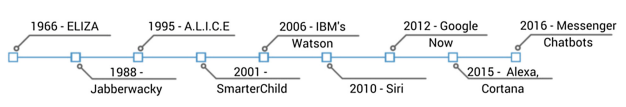
\includegraphics[width = 100mm]{chatbot-history}
	\caption{History of chatbots.}
	\label{chatbot-history}
\end{figure}

% \subsection{Rule-Based Bots}

% \subsection{AI Bots}






\subsubsection{Messenger Bots}
In April 2016, Facebook released their chatbot feature in Messenger. The main purpose was to increase people's experience with the platform and to let businesses reach out to their customers in a completely new way \cite{messenger}. To make it easier for developers and designers to build beautiful and consistent messenger bots that allows for a unified experience, Facebook released design guidelines to follow \cite{messenger_guidelines}. The messenger bot design guidelines are organized under three main headings:

\paragraph{Design Principles}
Facebook \cite{messenger_guidelines} suggest that bots should be brief. Since most people use messenger on their phone, interruptions should be expected. The easiest way to address this according to Facebook is to keep interactions short and concise. When that is not possible, developers and designers should consider how to maintain and reestablish context. Facebook \cite{messenger_guidelines} also advice to avoid modality; modality can create confusion and frustration for the users if they are interrupted in the middle of a task. Furthermore, conversations and graphical user interfaces (GUIs) should be mixed in the bots; Facebook offers a range of components, and these should be used depending on the bots functionalities and capabilities. It is also important to observe conversational norms and Facebook highlights the relevance to be deliberate about language, editorial voice, length of messages, and even speed of response. Embracing structure is also important when building a messenger bot. Making use of buttons, quick replies, and the persistent menu to structure user interactions while clearly communicating expectations. Moreover, Facebooks highlights the importance of developing a bot that notifies with care, fails gracefully, and is predictable in its interactions.

\paragraph{Language \& Editorial Voice}
Because bot interactions take place on Messenger, a messaging platform, the words used are important in explaining the experience a bot provides and why people should use it. Thus, Facebook suggest methods for writing interactions and best practices \cite{messenger_guidelines}. As writing best practices they suggest that it is important to preserve a voice, set user expectations, and to provide context. The bots voice or way of communication reflects its personality; it is essential to be consistent with it, in a tone that feels natural and human. It should also be easy for users to know what the bot can, or can not do, in order to set the correct user expectations. Further, bots should be as descriptive as possible to communicate core functionality; to build an understanding of the experience the bot creates, content should guide users every step of the way. Facebook also suggest designers and developers to design conversations before launching a chatbot. This can be done by starting to build a library of prompts and responses. According to them it is important to think about the goals and possible outcomes of a conversation, they also emphasis on creating a list of keywords to really get an overview of terms associated with the bot. Facebook also believe that mapping out interactions is a good idea, mapping gives a good overview of the tasks, expectations and contexts to establish with the bot. User responses can later be used to expand functionalities and capabilities \cite{messenger_guidelines}.

\paragraph{Tips for Sounding More Conversational}
In the end of their guidelines, Facebook gives tips on how to sound more conversational in writing. They emphasize on the importance of the chatbots style of writing; it has to converse in a way that its utility is not misrepresented or core capabilities are misunderstood. Furthermore, Facebook state that a conversational tone should support an experience, not define it \cite{messenger_guidelines}. They give some simple suggestions in how to implement a conversational tone in a chatbot by using an active voice, contractions of words, write in first and second person, to be careful with grammar and punctuation, and lastly the usage of a certain tone. The chatbots voice is its personality and the tone is how that personality is expressed \cite{messenger_guidelines}.

\subsection{Chatbots for Businesses}
The communication between brands and their clients has never been so intense as nowadays. With the rapid development of technology, the customer experience is changing dramatically. Customers want more autonomy and self-service options, preferring to make a purchase or get information without interacting with the human representative of the brand. In order to fit the expectations of their customers, companies are reshaping the experience from human-to-human interactions into the advanced self-service experience. Therefore, the use of chatbots in business can be a crucial issue of improving customer communication. Companies are using this technology to create a better engagement with their clients with the help of messaging platforms that offer a regular chat function, in-message purchases, and many other advanced functions.

\paragraph{Customer Service}
Most chatbots are general purpose, i.e., they attempt to hold open conversations in no specific area. Clearly this seems like a very difficult task computationally. But what if the scope was restricted ? Would chatter bots be able to perform better ? Indeed, these chatter bots exist in many forms, from website navigation assistants, to software virtual helpers, to gaming agents deployed extensively in massively multiplayer online role playing gaming engines, to more recognizable ones like Siri on Apple’s mobile platform. These bots typically would operate, i.e., hold conversations in a domain restricted to the company that was deploying them. Thus, their task should appear to be less computationally challenging than general purpose \cite{chakrabarti2015}.

\begin{figure}[htb]
	\centering
	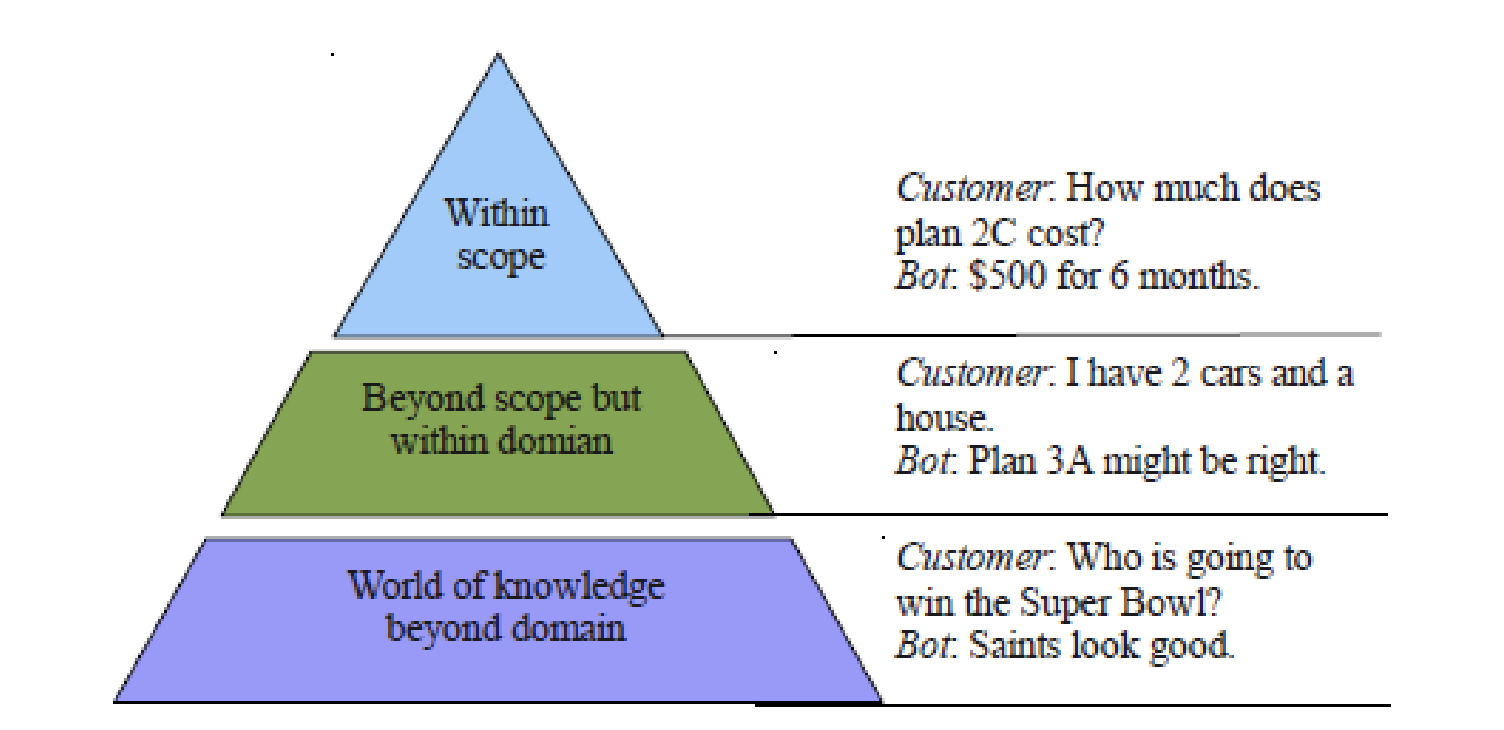
\includegraphics[width = 100mm]{conv-classes}
	\caption{Classes of Conversations: Within scope denoting specific conversations
within the domain, beyond scope denoting non-specific open-ended conversations
within the domain, and Beyond domain denoting conversations beyond the domain
being considered \cite{chakrabarti2015}.}
	\label{classes-of-conversations}
\end{figure}

Consider a snippet of conversation with a customer service chatter bot that helps customers solve account access issues. In this exchange, the customer is unable to login to an account, and seeks assistance \cite{chakrabarti2015}.
  \bigskip

{\fontfamily{cmss} \selectfont

  \color{red}
  \textbf{Chatter Bot}: Hello. How can I help you today ?
  \bigskip
  
  \color{blue}
  \textbf{Customer}: I am unable to login to my account. I forgot my password.
  \bigskip
  
  \color{red}
  \textbf{Chatter Bot}: Please click on the "Forgot Password" link. You will be emailed a link that will help you change your password.
  \bigskip
  
  \color{blue}
  \textbf{Customer}: I already tried that. That link takes me to a form to reset password. But it requires me to enter my Customer Relationship Number. I do not have this number.
  \bigskip
  
  \color{red}
  \textbf{Chatter Bot}: The Customer Relationship Number can be found in the "Account Information" tab when you log in to your account.
  \bigskip
  
  \color{blue}
  \textbf{Customer}: But I am unable to login to my account. I do not remember my password.
  \bigskip
  
  \color{red}
  \textbf{Chatter Bot}: Please click on the "Forgot Password" link. You will be emailed a link that will help you change your password.
  \bigskip
  
  \color{black}
}

To a human representative, it would be clear that this conversation is not helping address the customer’s issue. However, since chatter bots are programmed through pattern-template pairs, they are more suited for question-answer type exchanges, where there is a sequence of several question-answer pairs. They are unable to hold a longer conversation, understand the conversation, gauge whether the conversation is going in the desired direction, and act on it. In the above example, we expect the chatter bot to recognize the deadlock situation for the customer and to resolve it, or transfer the conversation to a human representative if the solution is beyond its programmatic capabilities.

It is clear from the example that the conversational performance of these chatter bots does not live up to what we would expect from a human customer service agent. Hence, there is clearly an opportunity to improve their conversational ability. In addition, since chatter bots cannot actually follow a longer conversation, they are also incapable of spotting opportunities in a conversation for providing unsolicited but pertinent information.


